%!TEX root = ../main.tex
%%%%%%%%%%%%%%%%%%%%%%%%%%%%%%%%%%
% Links:
%
% Difficulty:
% Companies: 
%%%%%%%%%%%%%%%%%%%%%%%%%%%%%%%%%%

\chapter{Coin Change Problem}
\label{ch:coin_change}
\section*{Introduction}

\begin{wrapfigure}{r}{0.5\textwidth}
    \vspace{-20pt}
    \begin{center}
        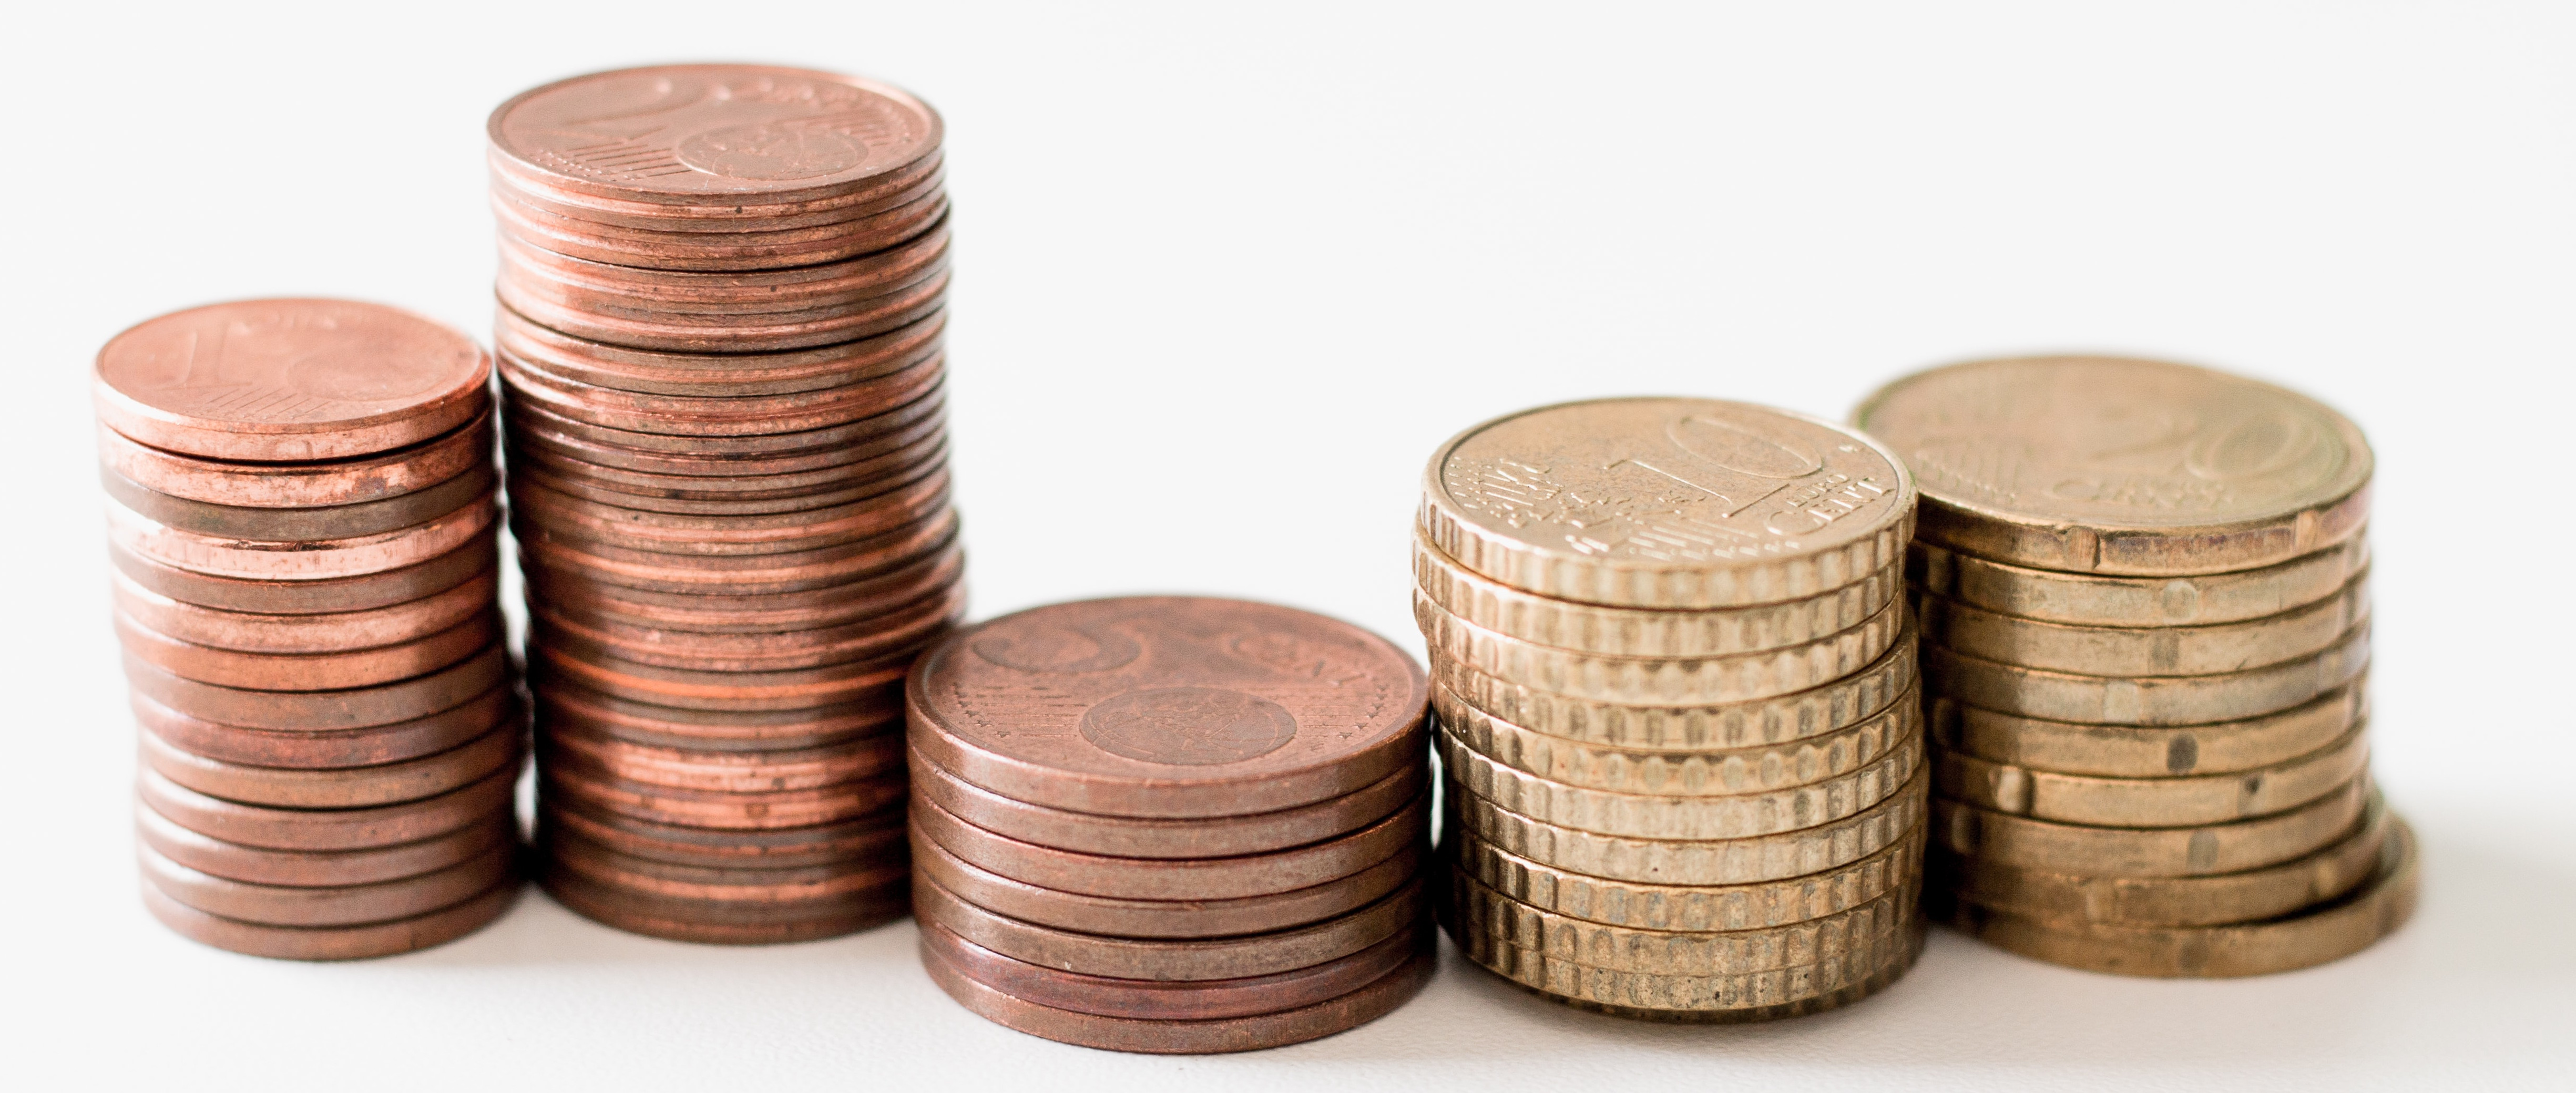
\includegraphics[width=0.48\textwidth]{sources/coin_change/images/coin_stacks}
    \end{center}
    %\vspace{-20pt}
    %\caption{A gull}
    \vspace{-15pt}
  \end{wrapfigure}
The problem discussed in this chapter is considered by many to be a fundamental stepping stone for anyone on the path towards mastering Dynamic Programming (see Section \ref{sect:appendix:DP}).
This reputation originates from the fact that this problem encompasses all the crucial ingredients of any DP algorithm with the additional benefit of having a very intuitive statement as 
it features things like coins and change that are concepts we are all familiar with.

This problem addresses the question of finding the minimum number of coins that add up to a given amount of money. 
Many people, when reading the statement of this problem, are tempted to approach it greedily but, as we will see, this does not always (despite it actually often does) lead to the correct answer. 

The coin change problem can be seen as an archetype for a whole bunch of DP optimization problems that can be reduced and solved, using the techniques shown in this section (see Chapter \ref{ch:dice_rolls} and \ref{ch:can_jump}, for instance).

\section{Problem statement}
\begin{exercise}
Write a function that, given an array of coin denominations $I$ and an integer $t$ representing an amount of money, returns
the minimum number of coins (of any denomination in $I$) that are necessary obtain $t$. 
You have an infinite amount of coins of each denomination. 

	\begin{example}
		\label{ex:coin_change:example1}
		\hfill \\
		Given $I=\{1,2,5\}$ and $t=11$, the function returns $3$.
		We can change $11$ in many ways, but none of them uses less than $3$ coins:
		\begin{itemize*}
			\item \textbf{two} coins of denomination $5$, and
			\item \textbf{one} coin of denomination $1$.
		\end{itemize*}
	\end{example}

	\begin{example}
		\hfill \\
		Given $I=\{1,3,4,5\}$ and $t=7$, the function returns $2$.
		We can change $7$ by using 
		\begin{itemize*}
			\item \textbf{one} coin of value $3$ and
			\item \textbf{one} of value $4$.
		\end{itemize*}
	\end{example}

	\begin{example}
		\label{ex:coin_change:example3}
		\hfill \\
		Given $I=\{1,5,8\}$ and $t=12$, the function returns $4$.
		We can change $12$ by using
		\begin{itemize*}
			\item \textbf{two} coins of value $1$ and
			\item \textbf{two} of value $5$.
		\end{itemize*}
	\end{example}
\end{exercise}

\section{Clarification Questions}

\begin{QandA}

	\item Can $I$ be empty?
	\begin{answered}
		\textit{Yes.}
	\end{answered}

	\item Is $I$ sorted?
	\begin{answered}
		\textit{No, denominations in $I$ are not sorted.}
	\end{answered}

	\item Can we assume we can always change $t$ using the denomination in $I$?
	\begin{answered}
		\textit{No, and if that is the case the function should return $-1$.}
	\end{answered}
	
\end{QandA}

\section{Discussion}
\label{coin_change:sec:discussion}

\subsection{The greedy approach and why it is incorrect}
This is one of those problems that can trick inexperienced candidates into thinking about a greedy approach, especially when nudged by the examples given along with the statement that are crafted so that a greedy approach produces the optimal answer.

A greedy algorithm for this problem works by repeatedly picking the largest coin $I_k$ that is smaller than $t$, and repeating the process on a new target amount $t-I_k$ until we reach $0$.
Listing \ref{list:coin_change:greedy} shows a possible implementation of this algorithm.

If we apply this algorithm to the Example \ref{ex:coin_change:example1}  we see that initially $t=11$
and that the largest denomination $5$ is smaller that $t$. Therefore we pick it (in the code this is reflected in assigning the variable \inline{greedy_choice = *it}) and we decrease $t$ by the same amount.
Now, $t=6$ which is still larger than $5$. We pick $5$ again and $t = 1$.
At this point neither $5$ nor $2$ are smaller or equal than $1$ and we choose $1$ which is the only denomination that is smaller or equal than the current value of $t$.
Now $t=0$ and we can stop, after having used $3$ coins in total, which is optimal.

However if we try the same algorithm on the Example \ref{ex:coin_change:example3} we get the answer $6$ which is quite far off from the optimum $4$. 
This approach is also not complete as it fails to find a valid solution like in the case where $I=\{2,5,8\}$ and $t=12$. In this case the greedy algorithm returns $-1$, when it is perfectly possible to change the amount $12$ by using 
\begin{itemize*}
	\item \textbf{two} coins of value $5$ and,
	\item \textbf{one} coin of value $2$.
\end{itemize*}	

\lstinputlisting[language=c++, caption={Greedy solution which always try to use the largest coin we can. Notice tht this approach is incorrect and should not be used during an interview.},label=list:coin_change:greedy]{sources/coin_change/coin_change_solution_greedy.cpp}



\subsection{Fomulation as an optimization problem}
\label{coin_change:sec:mathdefinition}
This problem can be formalized as an optimization problem where the solution is a set of number $X=\{x_0,x_1,\ldots, x_{|I|-1}\}$ of size $|I|$ with each $x_j$ representing how many coins of the denomination $I_j$ are used. 
Given this formulation, the answer is simply the minimum of Equation \ref{eq:coin_change:totalsum} subject to Equation \ref{eq:coin_change:totalsum_constraint}.
\begin{subequations}
\begin{equation}
	W(t) = \sum_{j=0}^{|I|-1} X_j
	\label{eq:coin_change:totalsum}
\end{equation}

\begin{equation}
	\sum_{j=0}^{|I|-1} X_j I_j = t
	\label{eq:coin_change:totalsum_constraint}
\end{equation}
\end{subequations}

$W(t)$ (Equation \ref{eq:coin_change:totalsum}) is the total  number of coins used and the constraint $W(t)$ is subject to (Equation \ref{eq:coin_change:totalsum_constraint}) forces their collective value to be exactly equal to the target amount $t$.

\subsection{Brute-force}
\label{coin_change:sec:bruteforce}
The brute-force approach is conceptually straightforward and consists in enumerating and checking every single possible valid combination of coins
while keeping track of the one with the fewest number of coins adding up to $t$.
A valid combination is described by an instance of the  array $X$ mentioned above in Section \ref{coin_change:sec:mathdefinition}.

The enumeration process can be implemented using recursion and backtracking. 
The idea is that we fill $X$ (which initially is zeroed) incrementally, by starting with the first position, $X_0$.
A value in $X$ at position $j$ ($x_j$) represents the number of coins of the denomination $I_j$ (contributing for a total value of $I_j X_j$). 

When we try a new value $k$ for $x_0$, we know we are adding $kI_0$ to the overall value of all the coins in $X$, and of course also that we used $k$ more coins.
Once a decision regarding the number of coins of value $I_0$ we use is made, we can continue and try to fill the next position of $X$ knowing that we have to make up for $t-(kI_0)$ and that we have used already $k$ coins. 

This process can be repeated until either we reach a point where we have nothing to make up for anymore, or we still have some amount left to change but, no available denominations to use.
In the former case we return the number of coins used up to that point (or we compare it to the current minimum so far), while in the latter, we return a value indicating that there is no solution (usually a large number).

An implementation of this idea is shown below in Listing \ref{list:coin_change:bruteforce}.
Notice that the function \inline{change_ways_bruteforce_backtracking_helper} takes $4$ parameters:
\begin{enumerate}
	\item \inline{I}: a read-only parameter containing the denominations;
	\item \inline{t}: the amount we need to make up for;
	\item \inline{j}: the index of the denomination in $I$ we are currently processing;
	\item \inline{coin_used}: the number of coin used so far.
\end{enumerate}


\lstinputlisting[language=c++, caption={Backtracking recursive brute-force solution},label=list:coin_change:bruteforce]{sources/coin_change/coin_change_solution3.cpp}

The function is initially called with $j=0$ (indicating we start with the first denomination), \inline{coin_used = 0} (no coins are used) and \inline{t} is set to be equal to the original amount (the one coming from the main driver function \inline{change_ways_bruteforce}).
As the execution and the recursion unfold, $t$ is changed accordingly to the value of the $k$ coins of denomination $I_j$ we are trying to use, \inline{coin_used} is incremented by $k$, and $j$ is incremented by one.

Figure \ref{fig:coin_change:recursiontree} shows the recursion tree of \inline{change_ways_bruteforce_backtracking_helper} 
when the input is the one shown in Example \ref{ex:coin_change:example1}; As we can see, there are $4$ ways (highlighted in \textcolor{darkgreen}{green}) of changing $4$ by using coin of denominations $\{1,2,3\}$:
\begin{enumerate}
	\item $2+2$ (two coins of value $2$),
	\item $1+3$, (one and three coins of values $1$ and $3$, respectively)
	\item $1+1+2$, (two and one coins of values $1$ and $2$, respectively), and
	\item $1+1+1+1$ ($4$ coins of value $1$).
\end{enumerate}
\begin{figure}
	\centering
	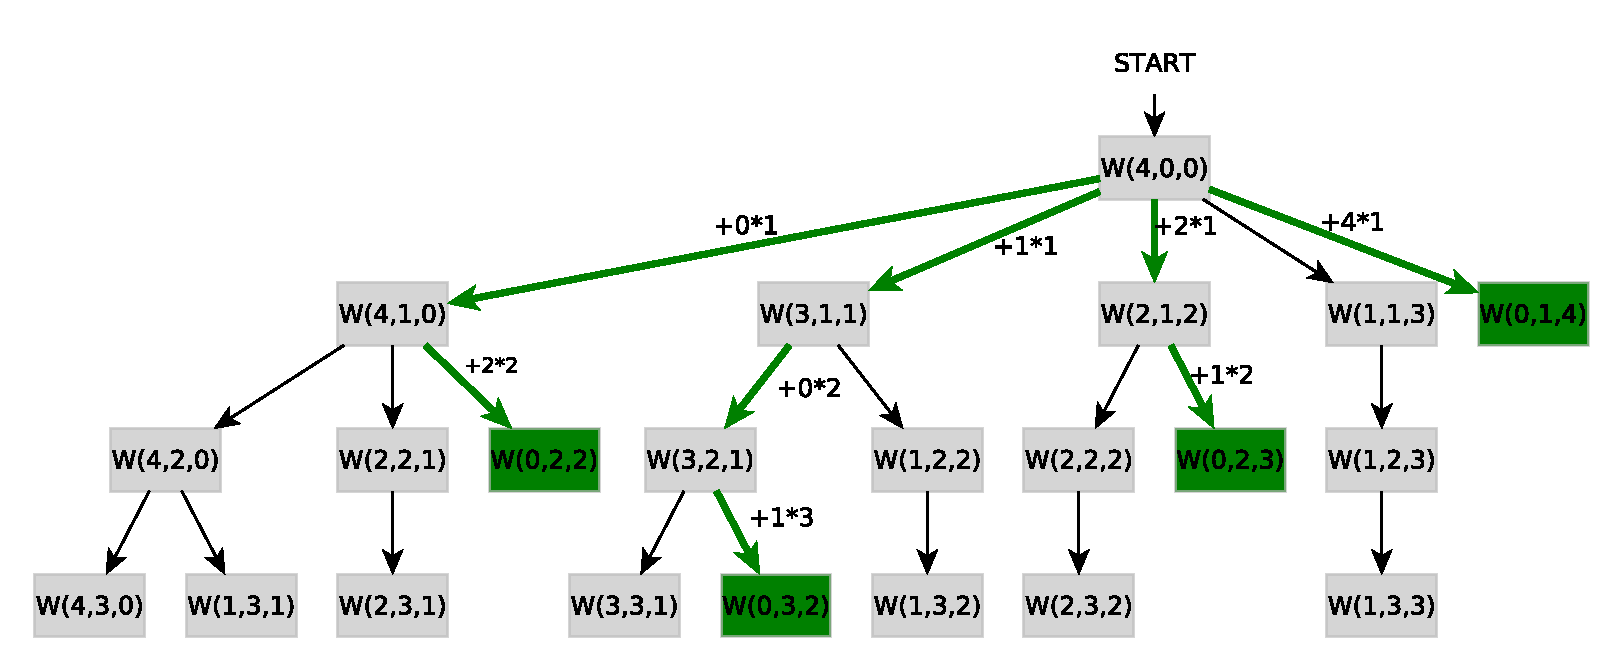
\includegraphics[width=\textwidth]{sources/coin_change/images/recursiontree}
	\captionsetup{singlelinecheck=off}
	\caption{This figure shows the call tree for the recursive function \inline{change_ways_bruteforce_backtracking_helper} on the following input:  $I = \{1,2,3\}$, and $t=4$. Each node contains the only three varying parameters of \inline{change_ways_bruteforce_backtracking_helper} (shortened here as $W$): the first is the current $t$ (the amount that we still need to make up for). The second   is the index to an element of $I$ for the denomination we are considering and the third is the number of coins used so far.
	Moreover, the highlighted paths shows all the valid ways of changing $4$. Note that all the green nodes have the first number equal to zero.}
	\label{fig:coin_change:recursiontree}
\end{figure}

The time complexity of this approach is exponential in $|I|$. 
As an informal proof of this fact consider that for each denomination we at least try either to use zero or one coin. 
Therefore for each element of $I$ we have two choices resulting in $2^{|I|}$ possibilities. 
The space complexity is linear in $|I|$ as in the worst case the depth of the recursive calls do not go deeper than $|I|$. This is a direct consequence of the base case, checking for $j >= |I|$.

\subsection{Dynamic Programming - Top-Down}
\label{sec:coin_change:topdown}
Like all DP problems, one of the first things we need to do, is to try to define the solution to the problem in terms of solutions to sub-problems
\footnote{The concept of sub-problem, in the context of this problem might seem quite fuzzy; You can think of it as a problem exactly equal to the main one except it operates on an input that
is  somehow \textit{\quotes{smaller}} and it is therefore easier to solve.
In this specific case it means $t$  is smaller.}.
Once that is in place, we need to make sure that our formulation satisfies the \textit{optimal substructure} property and, crucially, that also requires the solutions to the same sub-problems
more than once (see Appendix \ref{sect:appendix:DP}). 
Only then we are ready to unleash the full power of DP.

Consider the denominations listed in $I=\{I_0 < I_1 < \ldots \}$ and the function $C(x)$ which returns the minimum number of coins necessary to obtain the amount $x$ using $I$. 
We can calculate the value of $C(y)$ where $y > x$ very easily by using Equation \ref{eq:coin_change:dpformula}:
\begin{equation}
	\begin{cases}
		C(0) = 0 \\
		C(y) = +\infty \: \: \text{if} \: \: x < 0 \\
 		C(y) = 1 + \min_{d \in I} C(y-d)
	 \end{cases}
	\label{eq:coin_change:dpformula}
\end{equation}
We can see see that, the answer for the amount $y$ can be expressed in terms of answers to amount strictly smaller than $y$ and in particular, when:
\begin{itemize}
	\item $y=0$, the answer is $0$ as there is only one way of making up for the amount $0$ i.e. using zero coins;
	\item $y<0$ the answer is $+\infty$, signalling it is impossible to obtain a negative amount by only using positive denominations;
	\item in all the other cases, you can calculate the answer by using the answers to sub-problems for smaller amounts that you can obtain by subtracting the current amount with one of the coin denomination in $I$.
\end{itemize} 
The key point here is that $C(y)$, as it is defined in Equation \ref{eq:coin_change:dpformula} satisfies the optimal substructure property.
In-fact we can see that we can obtain the optimal answer to $C(y)$ from the optimal solution to smaller sub-problems. 

Moreover, if we apply Equation \ref{eq:coin_change:dpformula} to the Example \ref{ex:coin_change:example1} we see that solution to sub-problems are required over and over again:
\begin{itemize}
	\item $C(11) = \min(C(10),C(9), C(6))$
	\item $C(10) = \min(C(9),C(8), C(5))$
	\item $C(9) = \min(C(8),C(7), C(4))$
	\item $C(8) = \min(C(7),C(6), C(3))$
	\item $C(7) = \min(C(6),C(5), C(2))$
	\item $\ldots$
\end{itemize}
Figure \ref{fig:coin_change:DPtree} shows the initials layers of the recursion tree for $C(11)$, from which is it clear that the whole work described by the subtree $C(9)$ is done twice: once from  $C(11)$ when using a coin of value $2$ (\textcolor{red}{red} nodes) and a second time from $C(10)$ when using a coin of value $1$ (\textcolor{orange}{orange} nodes).

\begin{figure}
	\centering
	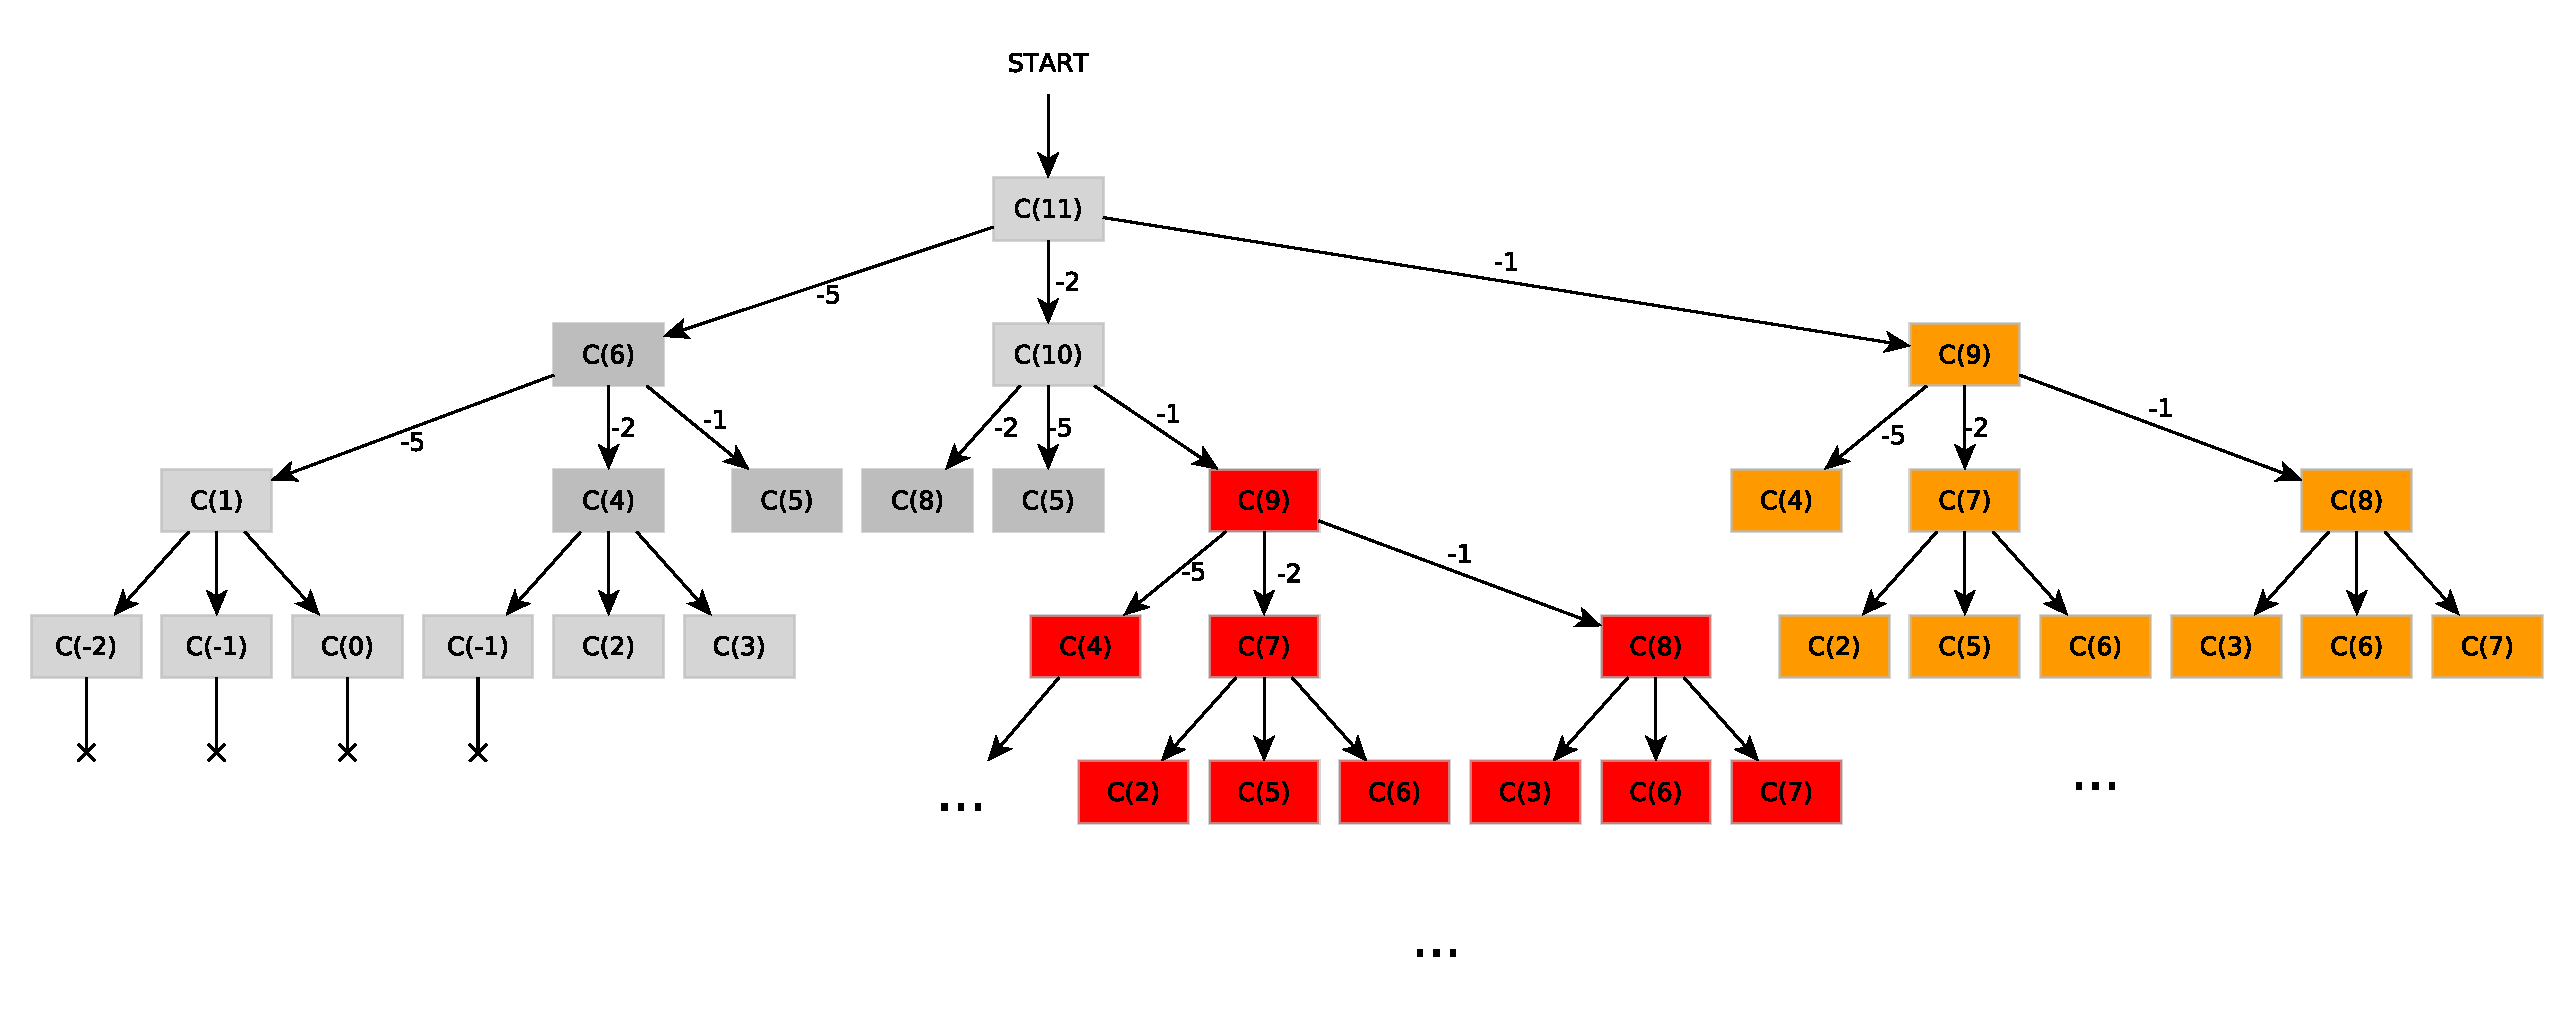
\includegraphics[width=\textwidth]{sources/coin_change/images/DPtree}
	\caption{Initial layers of the recursion tree for $C(11)$}
	\label{fig:coin_change:DPtree}
\end{figure}

Therefore, it seems that this problem also satisfies the overlapping subproblem property and we can very easily turn Equation \ref{eq:coin_change:dpformula} into an efficient DP solution by translating it into a memoized recursive function implementation as shown in Listing \ref{list:coin_change:topdown}.
The code works by blindly following what dictated by Equation \ref{eq:coin_change:dpformula} with the only addition of the function \inline{change_ways_DP_topdown_helper} being memoized via a cache, which takes the shape of a standard \inline{std::unordered_map}.

\lstinputlisting[language=c++, caption={Dynamic Programmin top-down solution.},label=list:coin_change:topdown]{sources/coin_change/coin_change_solution4.cpp}

The time complexity of Listing \ref{list:coin_change:topdown} is $\Theta(t|I|)$: There are $t+1$ possible  distinct calls to \inline{change_ways_DP_topdown_helper} and each of them costs 
$\Theta(|I|)$. The space complexity is $O(t)$ (if you consider the additional space occupied the  by the stack during the recursive process, otherwise it is constant); if $1 \in I$ then we get calls to \inline{change_ways_DP_topdown_helper} for every value from $t$ to $0$.

\subsection{Bottom-up}
\label{coin_change:sec:bottomup}
In Section \ref{sec:coin_change:topdown} we have seen how it is possible to use DP to attach and solve this problem efficiently by adopting a top-down approach. All DP solutions can be also implemented in a bottom-up fashion where we explicitly fill in a DP table ($T$) starting with the known values, usually corresponding to the base cases of the recursion for the top-down formulation.

Let's start by isolating the values of $t$ for which the solution is known. 
A good starting point seems to be the base cases of Listing \ref{list:coin_change:topdown} where $t=0$ and we return $0$ immediately. The next question we want to ask ourselves is, how can we fill cells of the DP table corresponding to higher values of $t$ starting from the value for the cell at $t=0$? The key idea here is that from a given $t$ we can obtain all the amounts corresponding to: $t+I_0,t+I_1,\ldots,  $ with a number of coins equal to the number of coins you needed to obtain $t$ plus $1$.

For instance if $I=\{1,2,5\}$ the DP table $T$ initially is as follows: $T=\{0,+\infty,+\infty,\ldots\}$.
From the value $0$ we can update cells for $t=1,2,5$ with the value $1$ and the the table becomes: $T=\{0,1,1,+\infty,+\infty,1,+\infty,\ldots\}$.
We can now repeat the process from $t=1$ and update all the values you can achieve from $t=1$ i.e. $2,3,6$. 
Notice that we can skip values $2$ and $3$  because they have already been obtained from the amount $1$ with fewer coins. 
$T$ is now: $T=\{0,1,1,2,+\infty,1,1,+\infty,\ldots\}$.
This process can continue until we have finished processing all the values up to $t$ and the final answer will be stored in the DP table cell for the amount $t$. 

More generally, assuming the table is filled up to (and including) cell at index $x+1$ (corresponding to the amount $x$)
you can update the cell of $T$ at index $0 \leq k < |I|$ as follows: $$T_{x+I_k} = \min (T_{x+I_k}, T_{x}+1)$$. 

Listing \ref{list:coin_change:bottomup} shows an implmentation of this idea. The time and space complexities are both $O(|I|\times t)$. 


\lstinputlisting[language=c++, caption={Dynamic Programmin bottom-up solution.},label=list:coin_change:bottomup]{sources/coin_change/coin_change_solution5.cpp}

\subsection{Conclusion}
In this chapter we have seen how to solve the Coin change problem which is a classical DP problem. 

The nice thing about this approach is that, we can reuse it virtually for any DP problem, provided we came up with a suitable recursive definition for the solutions to the subproblem.  All it is necessary is to code such a definition into a recursive function and use memoization to save precious computation steps. You can see more examples of problems solved with a similar techniques in Sections \ref{sect:appendix:DP},\ref{dice_rolls:sec:DP}, \ref{sec:max_manhattan:topdown}, \ref{sec:min_difficulty_job_scheduler_solution:dptopdown}, 
\ref{sec:palindrome_partitioning2:dptopdownimproved} and \ref{sec:square_in_matrix:top_down}

\section{Common Variations}

\subsection{Count the number of ways to give change.}
There is a very common variation of this problem where you are asked to return the total count of the possible ways you can change a given amount $t$. The solution approach
is the same and you can apply everything we have covered in this Chapter so far to solve this variant. 

\begin{exercise}
Write a function that given an array of coin denominations $I$ and an integer $t$ representing an amount of money, returns
the number of ways you can make up that amount by using coins of the denomination specified by the array $I$. 
You have an infinite amount of coins of each denomination. 
		\begin{example}
			\label{ex:coin_change:example1}
			\hfill \\
			Given $I={1,5,10}$ and $t=8$, the function returns $2$.
			We can change $8$ in two distinct ways:
			\begin{enumerate}
				\item eight coins of denomination $1$, or
				\item three and one coin of denomination $1$ and $5$, respectively.
			\end{enumerate}
		\end{example}
	
		\begin{example}
			\hfill \\
			Given $I={2,5,3,6}$ and $t=10$, the function returns $5$.
			We can change $8$ in the following ways:
			\begin{enumerate}
				\item five coins of denomination $2$,
				\item two and three coins of denomination $2$ and $3$, respectively,
				\item two and one coin  of denomination $2$ and $6$, respectively,
				\item one coin of the denominations $2$, $3$ and $5$, and finally,
				\item two coins of denomination $5$.
			\end{enumerate}
		\end{example}
\end{exercise}

